\documentclass[11pt]{article}

\usepackage[margin=1in]{geometry}
\setlength{\parindent}{0pt}
\usepackage{amsmath,amssymb,amsthm}
\usepackage{tikz}
\usetikzlibrary{arrows.meta, positioning}
\usepackage[numbers]{natbib}
\usepackage{subfigure}
\usepackage{graphicx}

\begin{document}

\title{Multi-Arm Trial Design with Distinct Biomarkers}
\author{}
\date{\today}
\maketitle

\section{Introduction and Motivation}

Biomarkers are variables that can be measured before treatment that are correlated to treatment outcome, ideally above standard of care. The idea in this brief is that we way to power a multi-arm RCT that validates promising biomarkers already reported in the literature. That is, the power calculation is powered to detect the significance of {\it biomarkers} themselves, rather than treatment effect across the population of study. The point of this is (1) to build off the work of others, as finding biomarkers from scratch could take even more sample size; (2) this would yield an excellent dataset from which to derive a post-hoc multiclass model that, using {\it all} biomarker data as inputs to a model, could determine which subset of treatments an individual is most indicated for.
\ \\

Let's now describe the setup for such a trial:

\begin{itemize}
\item \textbf{Randomization} into one of \(K\) experimental arms,
\item \textbf{Multiple biomarkers} \(\{X_1, \dots, X_K\}\), each potentially relevant to a specific experimental treatment,
\item \textbf{Outcome} \(Y\) (e.g.\ depression severity) measured post-treatment.
\end{itemize}

Our main goal is to evaluate, for each experimental treatment \(k\), whether the corresponding biomarker \(X_k\) \emph{predicts} an increased treatment effect. In turn, we'll develop the following:
\begin{itemize}
\item A simple causal model (DAG) for the multi-arm trial,
\item A linear model capturing main and interaction effects,
\item A data-generation scheme for simulation studies,
\item Methods for multiple testing and power analysis in this multi-biomarker context,
\item Empirical estimates of biomarker effects from literature,
\item Results from the power analysis, given these assumptions.
\end{itemize}

\pagebreak
\section{Model Setup}

\subsection*{DAG Representation}

We illustrate a basic causal structure for a multi-arm trial with randomization, treatments, correlated biomarkers, and outcome.

\begin{figure}[h!]
\centering
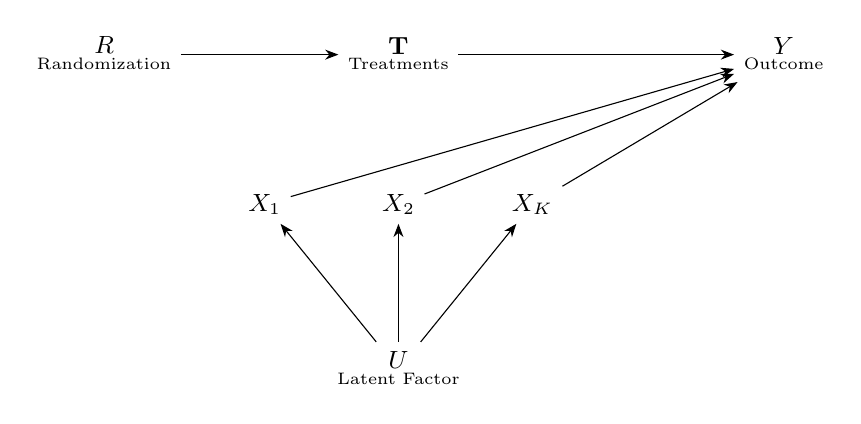
\begin{tikzpicture}[
  node distance=2.0cm,
  every node/.style={font=\small},
  >=Stealth
]
  % Nodes
  \node (R) {$\underset{\text{Randomization}}{R}$};
  \node (T) [right=of R] {$\underset{\text{Treatments}}{{\bf T}}$};
  \node (Y) [right=3.5cm of T] {$\underset{\text{Outcome}}{Y}$};

  % Biomarkers below T
  \node (X1) [below=1.3cm of T, xshift=-1.7cm] {$X_1$};
  \node (X2) [below=1.3cm of T] {$X_2$};
  \node (Xk) [below=1.3cm of T, xshift=1.7cm] {$X_K$};

  % Latent factor below X2
  \node (U) [below=1.5cm of X2] {$\underset{\text{Latent Factor}}{U}$};

  % Edges
  \draw [->] (R) -- (T);
  \draw [->] (T) -- (Y);
  \draw [->] (U) -- (X1);
  \draw [->] (U) -- (X2);
  \draw [->] (U) -- (Xk);
  \draw [->] (X1) -- (Y);
  \draw [->] (X2) -- (Y);
  \draw [->] (Xk) -- (Y);
\end{tikzpicture}
\caption{Simple DAG for a multi-arm trial with randomization node \(R\), treatments \(T\), optional latent factor \(U\) (introducing correlation among biomarkers), and outcome \(Y\).}
\label{fig:dag}
\end{figure}

\subsection*{Linear Model for the Outcome}

We assume a linear model capturing main effects of each treatment and possible interactions with corresponding biomarkers:
\[
\begin{aligned}
  Y_i \;=\;& \beta_0
  \;+\; \sum_{k=1}^K \Bigl[
      \beta_{1k}\,T_{ik}
    \;+\;\beta_{2k}\,X_{ik}
    \;+\;\beta_{3k}\,\bigl(T_{ik} \cdot X_{ik}\bigr)
  \Bigr]
  \;+\;\varepsilon_i,
  \\
  &\varepsilon_i \sim \mathcal{N}(0,\sigma^2),
\end{aligned}
\]
where:
\begin{itemize}
  \item \(\beta_0\) is the baseline intercept.
  \item \(\beta_{1k}\) is the \emph{main effect} of treatment \(k\) relative to an implicit baseline condition (e.g., the average of other arms, or arm 1 if using treatment contrasts).
  \item \(\beta_{2k}\) captures the baseline effect of biomarker \(X_k\) (assumed relevant to arm \(k\)), 
        with the understanding that \(\beta_{2k}\) can affect outcome under \emph{all} arms.
  \item \(\beta_{3k}\) measures the interaction (moderation) of treatment \(k\) by biomarker \(X_k\). 
        If \(\beta_{3k} > 0\), higher values of \(X_k\) predict greater treatment benefit for arm \(k\).
\end{itemize}
Note that because \(T_{ik}\) is binary and \(\sum_{k=1}^K T_{ik}=1\), every subject belongs to exactly one experimental arm.

\pagebreak
\section{Simulation Framework for Multi-Arm Trials}

To evaluate the operating characteristics of a multi-arm design that includes distinct biomarkers and treatments, one can simulate data as follows. Suppose there are \(K\) experimental arms, indexed by \(k=1,\dots,K\). Each subject \(i\) belongs to exactly one arm, indicated by the binary variables \(\{T_{i1}, \dots, T_{iK}\}\), with \(\sum_{k=1}^K T_{ik}=1\). We also have \(K\) biomarkers \(\{X_{1}, \dots, X_{K}\}\). Let \(N\) be the total number of subjects.

\begin{enumerate}
\item \textbf{Generate latent factor(s) (optional).} 
  If correlation among the biomarkers is desired, one or more latent factors can be introduced. 
  For instance, draw \(U_i \sim \mathcal{N}(0,1)\) for each subject \(i\). 
  Later steps can incorporate this factor into the biomarker generation process.

\item \textbf{Generate biomarkers.} 
  For each subject \(i\) and biomarker \(k \in \{1,\dots,K\}\), set
  \[
    X_{ik} \;=\; \mu_k \;+\; \gamma_k\,U_i \;+\; \sigma_{X_k}\,\eta_{ik}, 
    \quad \eta_{ik} \sim \mathcal{N}(0,1).
  \]
  Here, \(\gamma_k\) controls how strongly the latent factor \(U_i\) influences the \(k\)th biomarker, and \(\sigma_{X_k}\) scales any residual variation.

\item \textbf{Assign treatments.}
  Each subject is randomized into exactly one arm. 
  A convenient approach is to sample \(\{T_{i1},\dots,T_{iK}\}\) from a multinomial distribution with probabilities \((p_1,\dots,p_K)\), 
  so that one \(T_{ik}=1\) and the rest are 0. 
  Often, \(p_1 = \cdots = p_K = \frac{1}{K}\) for equal allocation.

\item \textbf{Generate the outcome.}
  Using the linear model
  \[
    Y_i \;=\; 
      \beta_0 
      \;+\; \sum_{k=1}^K \Bigl[
          \beta_{1k}\,T_{ik}
        \;+\;\beta_{2k}\,X_{ik}
        \;+\;\beta_{3k}\,\bigl(T_{ik} \cdot X_{ik}\bigr)
      \Bigr]
      \;+\;\varepsilon_i, 
    \quad \varepsilon_i \sim \mathcal{N}(0,\sigma^2),
  \]
  each subject's outcome depends on which experimental arm they are assigned to (\(T_{ik}=1\) for exactly one \(k \in \{1,\dots,K\}\)), 
  the values of the biomarkers \(\{X_{ik}\}\), 
  and the error term \(\varepsilon_i\). 
  The intercept \(\beta_0\) represents a baseline outcome level, 
  \(\beta_{1k}\) is the main effect of arm \(k\) (relative to an implicit baseline), 
  \(\beta_{2k}\) captures any overall effect of \(X_k\), 
  and \(\beta_{3k}\) is the interaction term indicating how biomarker \(X_k\) moderates treatment \(k\).

\end{enumerate}

By repeating this process for multiple simulated datasets, one can fit the same linear model 
\[
   Y \;\sim\; \{T_{1},\dots,T_{K}\} \;+\; \{X_{1},\dots,X_{K}\} \;+\; \{T_{k} \cdot X_{k}\}_{k=1}^K
\]
to each dataset and evaluate how often the estimated interaction terms \(\hat{\beta}_{3k}\) are statistically significant. 
This approach yields estimates of power, type~I error rate, or other design metrics, 
accounting for the correlation structure among biomarkers and multiple treatment arms.

\pagebreak
\section{Candidate Biomarkers and Empirical Estimates of Effects}

Below we consolidate and discuss illustrative findings from the literature, focusing on four candidate biomarkers that may moderate treatment response in depression. We present these examples to highlight the breadth of effect sizes, populations, and methodological nuances that can arise when designing multi-arm biomarker trials.

\subsection{Alpha Peak Frequency (iAPF) for rTMS}

Three studies have examined whether \emph{individual alpha peak frequency} (iAPF) predicts response to 10\,Hz or 1\,Hz rTMS protocols in Major Depressive Disorder (MDD), as well as to neurofeedback or medication in ADHD. Voetterl \textit{et al.}~(2019)~\cite{voetterl2023}, though focused on ADHD, reported that matching patients' iAPF decile to a particular intervention (methylphenidate vs.\ neurofeedback plus sleep coaching) yielded a sizable remission gain (on the order of 15--30\,\%). Roelofs \textit{et al.}~(2021)~\cite{roelofs2021} and Corlier \textit{et al.}~(2019)~\cite{corlier2019} studied MDD populations receiving rTMS, finding that \emph{proximity} of iAPF to the 10\,Hz stimulation frequency explained about 5--10\,\% of variance in symptom improvement (a correlation of about $r\approx -0.25$ for Roelofs, $r\approx 0.30$ for Corlier), whereas no effect was apparent in the 1\,Hz group or in patients who switched off 10\,Hz mid-treatment.

Although the exact magnitudes differ by population and methodology (and ADHD vs.\ MDD is an imperfect comparison), a recurring theme is that \emph{alignment} or \emph{closeness} between one's alpha peak and the rTMS frequency can moderate clinical outcome. Correlations in the range of 0.20--0.30 (i.e.\ explaining roughly 5--10\,\% of outcome variance) are consistent with a moderate interaction effect ($\beta_{3}\approx 0.2$--0.3 if the outcome is continuous). Stronger effects have been reported in some settings (e.g.\ ADHD). However, non-linear patterns (peaks around 10\,Hz rather than strictly linear) may matter, complicating a simple linear interaction model. Hence, an RCT seeking to confirm iAPF as a predictive biomarker for rTMS would likely assume at least a modest but clinically meaningful interaction size.

\vspace{1ex}
\noindent
\textbf{Caveats.} 
Voetterl's ADHD sample differs in population, comorbidity, and outcome measures relative to MDD rTMS trials. Corlier's retrospective design (with possible protocol switches) may attenuate effect estimates. Nonetheless, across all three studies, alpha-frequency alignment emerges as a plausible biomarker worthy of prospective validation.

\subsection{EHR-Based Predictors of Ketamine Response}

A series of four small-to-moderate trials~\cite{niciu2014,permoda-osip2014,luckenbaugh2012,phelps2009} found that \emph{family or personal history of alcohol use disorder (AUD)} predicts a more robust antidepressant response to ketamine in both MDD and bipolar depression. For instance, Niciu \textit{et al.}~(2015) reported that a combination of family history of AUD, BMI, and prior suicide attempt explained up to 36\,\% of variance in outcome by Day~7 post-infusion. Meanwhile, Permoda--Osip \textit{et al.}~(2014) and Luckenbaugh \textit{et al.}~(2012) observed that 45--60\,\% of responders (vs.\ about 15--20\,\% of non-responders) had a positive AUD history, corresponding to odds ratios around 3--5. Phelps \textit{et al.}~(2009) noted an absolute difference of nearly 50\,\% in response rates (67\,\% vs.\ 18\,\%), yielding an even larger odds ratio.

Such large contrasts suggest a potentially strong $\textit{treatment} \times \textit{AUD-history}$ interaction. In a logistic model, an odds ratio of about 3 corresponds to a log-odds coefficient $\ln(3)\approx 1.1$. Even if some estimates are inflated by small sample sizes or retrospective biases, these consistent findings highlight that certain EHR-derived variables can have substantial predictive value for ketamine response. A well-powered multi-arm trial (one of the arms being ketamine) that collects family/personal AUD data could detect this interaction with fewer subjects than is typically required for more modest biomarkers.

\vspace{1ex}
\noindent
\textbf{Caveats.} 
These results come from relatively small samples and mixed unipolar/bipolar populations. Confirmatory RCTs with strict randomization and larger $N$ are still needed to rule out confounding or selection biases. In practice, investigators might combine AUD history with other EHR factors into a multi-variable biomarker.

\subsection{Inflammatory Markers for ECT (Dellink et al., 2025)}

A recent meta-analysis by Dellink \textit{et al.}~(2025)~\cite{dellink2025} aggregated 14 studies of ECT in depression ($n\!=\!556$) and found that patients with higher baseline levels of \emph{C-reactive protein} (CRP) or \emph{interleukin-6} (IL-6) consistently showed greater symptom reduction from acute ECT courses. The effect, however, was modest: correlations of about $r\approx 0.20$, implying these markers explained about 4\,\% of the variance in outcomes. Changes in these markers \emph{during} the course of ECT did not correlate strongly with final outcomes, suggesting a potential \emph{trait-level} rather than \emph{state-level} predictive mechanism.

For multi-arm trials that include an ECT arm, this finding supports the possibility of an \emph{inflammatory-subtype} of depression that responds preferentially to ECT. Given $r\approx 0.20$, one can anticipate a smaller interaction coefficient (e.g.\ $\beta_{3}\approx 0.2$ in a standardized linear framework). Detecting such an effect reliably would likely demand a larger sample size than is needed for strong predictors like AUD history.

\vspace{1ex}
\noindent
\textbf{Caveats.}
Heterogeneity exists in how each study measured CRP/IL-6 and defined "high inflammation." The $n=556$ total still spans multiple ECT protocols and populations. Nonetheless, the consistent direction of effect (higher inflammation, better ECT response) warrants further prospective confirmation.

\subsection{Speech Latency as a Voice Biomarker (Siegel et al., 2024)}

Siegel \textit{et al.}~(2024)~\cite{siegel2024} explored \emph{speech latencies}---the time between interviewer and patient speech turns---in a 3-arm bipolar depression trial of SEP-4199 vs.\ two comparators. Baseline psychomotor slowing, captured by longer latencies, correlated with more robust improvement under the \emph{active} agent compared to placebo ($r\approx 0.30$). Patients with normal latencies tended to improve rapidly even on placebo, reducing any measured drug--placebo gap.

In a multi-arm design that includes a novel medication alongside other experimental treatments, such voice-based measures could be an inexpensive, objective biomarker. An observed partial correlation of 0.30 corresponds to about 9\,\% variance explained and a moderate $\beta_{3}\approx 0.3$ in a linear model. Because speech recording imposes minimal burden, it may be an attractive option for biomarker collection in large trials.

\vspace{1ex}
\noindent
\textbf{Caveats.}
Psychomotor slowing may not be the only driver of delayed turn-taking; anxiety, cognitive impairment, or environment (e.g.\ telehealth) could also influence latencies. Further validation in bigger samples is needed to confirm specificity for medication response. 

\bigskip

Overall, these four examples illustrate a range of plausible biomarker strengths and methodological complexity. Effect sizes vary from modest ($r\approx 0.20$) to quite large (odds ratios of 3--5). Different diagnostic groups (unipolar vs.\ bipolar depression, ADHD), sample sizes, and outcome measures each add layers of heterogeneity. For planning future \emph{multi-arm RCTs}, careful synthesis of these prior estimates, along with explicit simulation (as outlined in previous sections), can guide sample size requirements and statistical methods for reliably detecting treatment--biomarker interactions.

\pagebreak
\section{Multiple Testing and Power Analysis}

In a multi-arm, multi-biomarker setup, each $k=1,\ldots,K$ generates a hypothesis $H_{0,k}:\beta_{3k}=0$. To control the familywise error rate or false discovery rate, common adjustments include:

\begin{itemize}
\item \textbf{Holm's step-down (FWER):} Sort $p$-values in ascending order, apply successively stricter thresholds, and stop once a test fails rejection.
\item \textbf{Benjamini--Hochberg (FDR):} Sort $p$-values and apply a threshold that controls the false-discovery rate at $\alpha$.
\end{itemize}

One can define various \emph{success criteria}, for example:
\begin{itemize}
  \item \textbf{\texttt{any}} significant biomarker ($\exists k: p_k < \alpha^*$),
  \item \textbf{\texttt{all}} biomarkers significant ($\forall k: p_k < \alpha^*$),
  \item \textbf{Other subsets} (e.g.\ at least two biomarkers pass; unimplemented for now).
\end{itemize}

\subsection{Illustrative Simulation Results}

The following are the resulting power curves using the assumptions developed above.

\begin{figure}[htbp]
\centering
\subfigure[Biomarker power: BH]{
  \includegraphics[width=0.95\textwidth]{figs/biomarker_power_BH.png}
}
\subfigure[Biomarker power: Holm]{
  \includegraphics[width=0.95\textwidth]{figs/biomarker_power_holm.png}
}
\caption{Example per-biomarker power curves under BH and Holm corrections.}
\label{fig:biomarker_power}
\end{figure}

\begin{figure}[htbp]
\centering
\subfigure[Overall success (BH, \texttt{any}).]{
  \includegraphics[width=0.45\textwidth]{figs/overall_success_BH_any.png}
}
\subfigure[Overall success (BH, \texttt{all}).]{
  \includegraphics[width=0.45\textwidth]{figs/overall_success_BH_all.png}
}\\
\subfigure[Overall success (Holm, \texttt{any}).]{
  \includegraphics[width=0.45\textwidth]{figs/overall_success_holm_any.png}
}
\subfigure[Overall success (Holm, \texttt{all}).]{
  \includegraphics[width=0.45\textwidth]{figs/overall_success_holm_all.png}
}
\caption{Example overall success rates under BH vs.\ Holm correction, comparing 
two success criteria: \texttt{any} significant biomarker vs.\ \texttt{all} biomarkers significant.}
\label{fig:overall_success}
\end{figure}

\paragraph{Observations.}
\begin{itemize}
\item \textbf{Per-Biomarker Power} (Figure~\ref{fig:biomarker_power}) reveals stark differences in detection rates:
  \begin{itemize}
  \item The strongest biomarker (AUD history for ketamine, $\beta_{3}\approx 0.6$) achieves 80\% power with just 100 subjects per arm.
  \item Moderate biomarkers (iAPF for rTMS, $\beta_{3}\approx 0.3$) require 300--400 subjects per arm for similar power.
  \item Weaker biomarkers (inflammatory markers for ECT, $\beta_{3}\approx 0.2$) need 500+ subjects per arm.
  \end{itemize}

\item \textbf{Overall Success} (Figure~\ref{fig:overall_success}) shows dramatic differences between criteria:
  \begin{itemize}
  \item Under \texttt{any}, power grows rapidly once the strongest biomarker achieves moderate power, reaching 80\% with 300 subjects per arm.
  \item Under \texttt{all}, power is dominated by the weakest biomarker, requiring 2000+ subjects per arm to achieve 80\% power.
  \item The gap between \texttt{any} and \texttt{all} widens as sample size increases, reflecting the challenge of simultaneous detection.
  \end{itemize}

\item \textbf{Multiple Testing Methods} show minimal impact:
  \begin{itemize}
  \item BH and Holm corrections yield nearly identical power curves, especially under \texttt{any}.
  \item With only $K=4$ hypotheses, the numerical differences between correction methods are negligible.
  \item The choice of success criterion (\texttt{any} vs.\ \texttt{all}) matters far more than the correction method.
  \end{itemize}
\end{itemize}

\pagebreak
\section{Summary}

A multi-arm trial that evaluates distinct treatment--biomarker interactions can efficiently explore multiple hypotheses in a single protocol. Our simulation framework reveals several key insights for trial design:

\begin{itemize}
\item \textbf{Sample Size Requirements Vary Dramatically:}
  \begin{itemize}
  \item Strong biomarkers (e.g., AUD history for ketamine) can be validated with modest samples ($n\approx 100$ per arm).
  \item Moderate biomarkers (e.g., iAPF for rTMS) require 3--4x larger samples.
  \item Weak biomarkers (e.g., inflammatory markers) may need 5x larger samples.
  \end{itemize}

\item \textbf{Success Criteria Drive Design:}
  \begin{itemize}
  \item The \texttt{any} criterion is practical for exploratory trials, achieving 80\% power with 300 subjects per arm.
  \item The \texttt{all} criterion is extremely conservative, requiring 2000+ subjects per arm.
  \item Investigators should carefully consider whether detecting all biomarkers is truly necessary.
  \end{itemize}

\item \textbf{Multiple Testing is Secondary:}
  \begin{itemize}
  \item With few hypotheses ($K=4$), the choice between BH and Holm has minimal impact.
  \item The success criterion dominates the power analysis.
  \item More sophisticated corrections may be unnecessary in this context.
  \end{itemize}
\end{itemize}

Real-world biomarkers for TRD, such as iAPF alignment, alcohol-use history, inflammatory markers, or speech latencies, illustrate a range of plausible effect sizes. In practice, investigators should:
\begin{itemize}
\item Prioritize biomarkers based on prior evidence strength and clinical importance.
\item Consider whether detecting all biomarkers is necessary or if finding any significant biomarker is sufficient.
\item Use the simulation framework to explore different sample sizes and success criteria.
\item Be prepared for substantial sample size requirements if all biomarkers must be validated simultaneously.
\end{itemize}

By examining the resulting power curves, one can plan a multi-arm trial that is appropriately powered to detect meaningful biomarker--treatment interactions while balancing statistical rigor with practical feasibility.

\pagebreak
\bibliographystyle{plainnat}
\bibliography{bibliography}

\end{document}
